\section{Text recognition}

Goal: Transcription (ASCII or Unicode) of text. Analysis also covers language
and script recognition, font recognition, writer authentication, word spotting,
...

OCR good results for non-cursive printed text, clean images, high resolution.
Challenging for cursive script, continuous handwritten text, degraded
documents.

\subsection{Sayre's paradox}

With cursive text / connected characters, character recognition requires
character segmentation, and character segmentation requires character
recognition. Approaches: Recognize whole worlds, test multiple hypothesis,
combine the two.

\subsection{Processing steps}

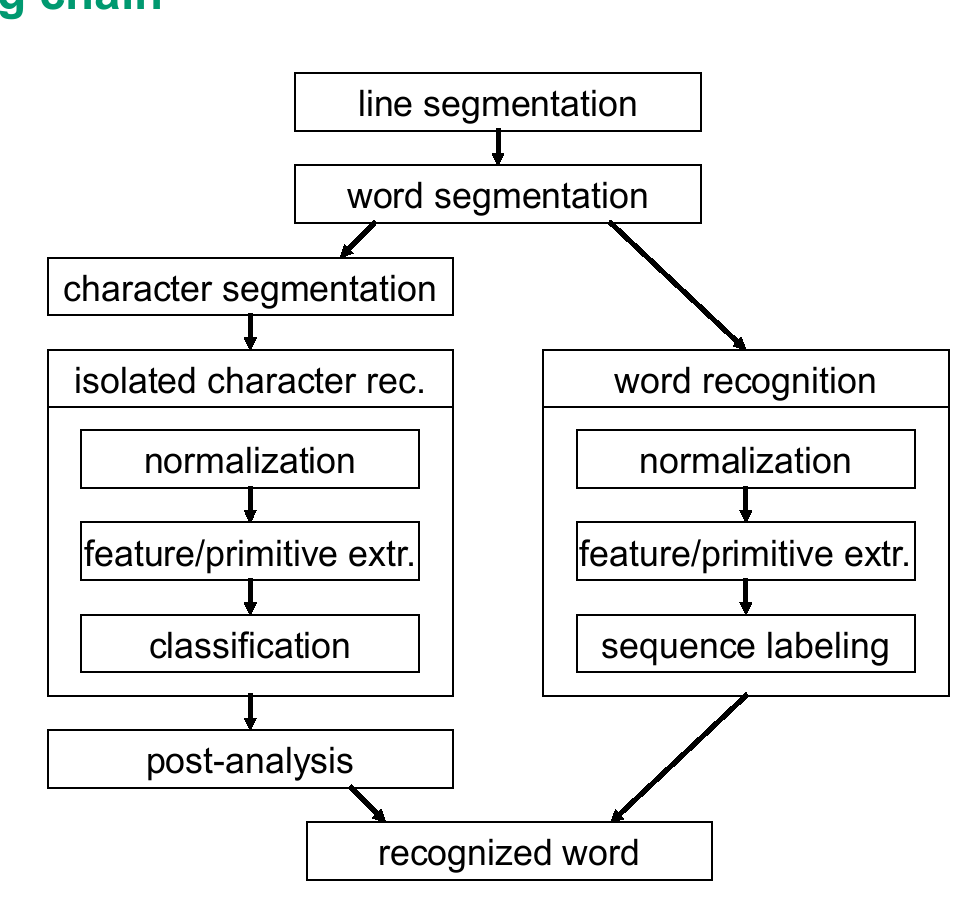
\includegraphics[width=0.5\textwidth]{07_processing}

\subsection{Character recognition}

\begin{itemize}
		\item Isolated character recognition applicable to high-quality printed
				text or constrained handwriting. Challenge: Variability of
				class.
		\item Classification: Statistical (KNN, SVM, ...), direct comparison
				with model, pattern recognition
		\item Similarity measures: Hamming distance, warping distance
		\item Two steps: Feature extraction, then classification
		\item Typical features: Dimensions, density, projection profiles, HOG,
				LBP, ...
\end{itemize}

\subsubsection{Structural approaches}

\begin{itemize}
		\item Shapes decomposed into strokes, properties extracted: Number of
				connected components, number of holes, concavities and
				convexities, ...
		\item These primitives represented as strings, trees, graphs and compared
\end{itemize}

\subsection{Classification}

\begin{description}
		\item[KNN] Sample classified by plurality vote of its neighbours (see
				which class majority of its $k$ nearest neighbours belong to)
		\item[MLP] Fully connected neural network with hidden layer, decision
				based on highest activation on output layer
		\item[SVM] Map initial feature space to augmented space where linear
				discrimination possible. Finds hyperplane with maximum
				separating distance between classes.
\end{description}

\subsection{Word recognition}

\begin{itemize}
		\item Alternative to character recognition, useful if limited
				vocabulary, language-driven approach or keyword spotting
		\item Typically used for cursive scripts, handwriting or
				difficult-to-segment scripts
		\item More possible cases, more features needed
		\item But can use external language knowledge, dictionaries, ...
		\item Feature extraction using sliding window
		\item Dynamic time warping, hidden markov models, ... suitable for
				sequential data analysis
\end{itemize}

\subsubsection{Dynamic time warping}

\begin{itemize}
		\item Calculates similarity between time series, based on DP
\end{itemize}

\subsubsection{Hidden markov model}

\begin{itemize}
		\item Class modeled by a two-stage stochastic process using hidden and
				visible state.
		\item Hidden model has states and transition function (think FSM).
				Observations linked to states via emission functions. Idea:
				Predict state via observations.
		\item That is pick state which best explains patterns in observations.
\end{itemize}
